\section{eo\-Perf2Worth$<$ EOT, Worth\-T $>$ Class Template Reference}
\label{classeo_perf2_worth}\index{eoPerf2Worth@{eoPerf2Worth}}
Base class to transform raw fitnesses into fitness for selection.  


{\tt \#include $<$eo\-Perf2Worth.h$>$}

Inheritance diagram for eo\-Perf2Worth$<$ EOT, Worth\-T $>$::\begin{figure}[H]
\begin{center}
\leavevmode
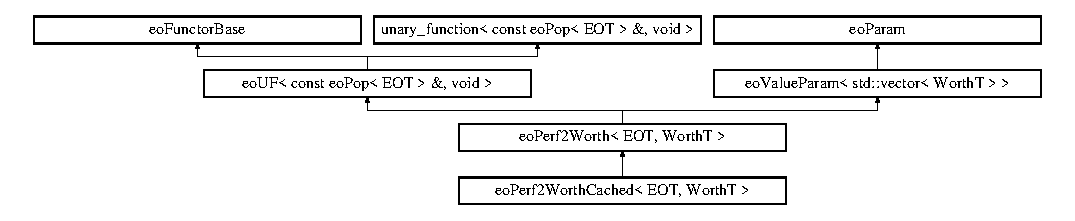
\includegraphics[height=2.52252cm]{classeo_perf2_worth}
\end{center}
\end{figure}
\subsection*{Public Member Functions}
\begin{CompactItemize}
\item 
{\bf eo\-Perf2Worth} (std::string \_\-description=\char`\"{}Worths\char`\"{})\label{classeo_perf2_worth_a0}

\begin{CompactList}\small\item\em default constructor \item\end{CompactList}\item 
virtual void {\bf sort\_\-pop} ({\bf eo\-Pop}$<$ {\bf EOT} $>$ \&\_\-pop)\label{classeo_perf2_worth_a1}

\begin{CompactList}\small\item\em Sort population according to worth, will keep the worths and fitness\_\-cache in sync with the population. \item\end{CompactList}\item 
virtual void {\bf resize} ({\bf eo\-Pop}$<$ {\bf EOT} $>$ \&\_\-pop, unsigned sz)\label{classeo_perf2_worth_a2}

\item 
virtual void {\bf operator()} ({\bf eo\-Pop}$<$ {\bf EOT} $>$ \&\_\-pop)\label{classeo_perf2_worth_a3}

\end{CompactItemize}


\subsection{Detailed Description}
\subsubsection*{template$<$class EOT, class Worth\-T = double$>$ class eo\-Perf2Worth$<$ EOT, Worth\-T $>$}

Base class to transform raw fitnesses into fitness for selection. 

\begin{Desc}
\item[See also:]{\bf eo\-Select\-From\-Worth}{\rm (p.\,\pageref{classeo_select_from_worth})} \end{Desc}




Definition at line 43 of file eo\-Perf2Worth.h.

The documentation for this class was generated from the following files:\begin{CompactItemize}
\item 
eo\-Perf2Worth.h\item 
fitness\_\-traits.cpp\end{CompactItemize}
